\documentclass[a4paper,14pt]{extarticle} \usepackage[utf8]{inputenc}
\usepackage[T1]{fontenc}
\usepackage[margin=2.5cm]{geometry}

% Fonte Caladea se existir, senão lmodern
\IfFileExists{caladea.sty}{
  \usepackage{caladea}
}{
  \usepackage{lmodern} }
\usepackage{ragged2e}
\usepackage{graphicx}
\usepackage[portuguese]{babel}
\usepackage{wrapfig}
\usepackage{hyperref}
\usepackage{fancyhdr}
\usepackage{xcolor}
\usepackage{rotating}
\usepackage{titlesec}
\usepackage{epigraph}
\usepackage{dirtytalk}
\usepackage{indentfirst} % Indenta o primeiro parágrafo após seções

% Ajuste do recuo de parágrafo
\setlength{\parindent}{1.5em}

% Centralizar títulos
\titleformat{\section}
  {\normalfont\centering\bfseries\Large}{\thesection}{1em}{}

\titleformat{\subsection}
  {\normalfont\centering\bfseries\large}{\thesubsection}{1em}{}

\titleformat{\subsubsection}
  {\normalfont\centering\bfseries}{\thesubsubsection}{1em}{}

% -------------- Símbolos de Versículo e Resposta --------------
% Definição do símbolo (a “barrinha” inclinada)
\makeatletter
\newcommand{\vers@resp@sym}{%
  \raisebox{0.2ex}{\rotatebox[origin=c]{-20}{$\m@th\rceil$}}%
}
% macro interna que sobrepõe a barrinha e a letra V ou R
\newcommand{\vers@resp}[2]{%
  {\ooalign{%
     \hidewidth\kern#1\vers@resp@sym\hidewidth\cr
     #2\cr
  }}%
}
% comandos públicos \versicle e \response
\DeclareRobustCommand{\versicle}{\vers@resp{-0.1em}{V}}
\DeclareRobustCommand{\response}{\vers@resp{0pt}{R}}
\makeatother
% ^------------- Símbolos de Versículo e Resposta -------------^

% Rodapé com imagem e página
\pagestyle{fancy}
% ---- Cabeçalho ------------
\fancyhf[C]{}
% ----- Rodapé --------------
\fancyfoot[LO,LE]{%
  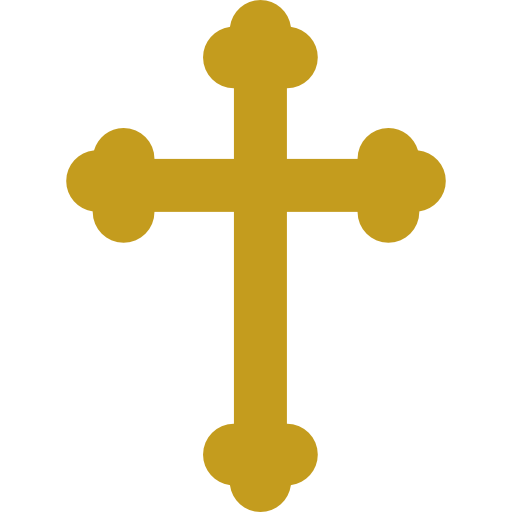
\includegraphics[scale=0.2]{assets/cross.png}\quad
  \textit{Novena a \textbf{Beata Sandra Sabattini}}
}
\fancyfoot[RO,RE]{\thepage}

\begin{document}


\subsection*{Novena a Beata Sandra Sabattini}


``<<Sandra foi uma autêntica artista>> , acrescentou o cardeal Semeraro, porque “aprendeu muito bem a linguagem do amor, com as suas cores e sua musicalidade”. A sua santidade foi “abrir-se à partilha com os últimos, o colocar ao serviço de Deus toda a sua jovem existência terrena, feita de entusiasmo, simplicidade e grande fé.''
\par\noindent\rule{\textwidth}{0.4pt}

\tableofcontents
\thispagestyle{empty}

% --- Vida / Origem da Novena ---
\newpage


% --- Orações Diárias ---
\newpage
\section{Novena a Beata Sandra Sabattini}
\subsection{Oração Inicial para todos os dias}

"Não sou eu que procuro Deus, mas é Deus que me procura.” Beata Sandra Sabattini, da mesma forma que buscastes um constante contato com Deus, busco neste momento estar em profunda oração. Seja minha intercessora e me ensine esse profundo amor que tens a Deus e a testemunhar com alegria. Desça sobre mim o Espírito Santo, para que eu adore a Deus verdadeiramente nesta novena.

 “A caridade é a síntese da contemplação e da ação, é o ponto de encontro entre o céu e a terra, entre o homem e Deus”. Tal como vossa serva Sandra, desejo esperar ativamente em Deus, com todo esforço da minha alma, as graças dessa intimidade de 9 dias de novena.


\subsection{1º Dia de Novena:} "Se eu não fizer uma hora de oração por dia, eu nem me lembro de ser cristã." (Beata Sandra Sabattini)

“Ela levantou cedo, no início da manhã, para se encontrar sozinha na meditação, talvez no escuro, em frente ao Santíssimo Sacramento, antes que outros chegassem à igreja. – relata seu tio Don Giuseppe – No primeiro dia do ano, de uma a duas da manhã, ele estava diante de Jesus em adoração. Ela adorava orar sentado na terra, como um sinal de humildade e pobreza."

Dê-nos, Senhor, Sandra como irmã, para nos acompanhar em nossa jornada de santificação.

Beata Sandra Sabattini, ensinai-me a humildade e perseverança da vida de oração.


\textbf{\textbf{1 Pai-Nosso, 3 Ave-Marias,  1 Glória ao Pai.}}


\subsection{2º Dia de Novena:} "Conformar com a vida de Jesus e compartilhar diretamente a vida do mínimo, colocar a vida com a deles e tomar conta de sua situação".(Comunidade Papa João XXIII)

Sandra em seus primeiros anos de vida teve influência de sua família cristã, em especial de seu tio Dom Giuseppe Bonini. Na Comunidade Papa João XXIII, esteve na companhia de Dom Oreste Benzi, um grande amigo de caminhada. Sandra era bem acompanhada pelo seu diretor espiritual padre Nevio Faitanini. Sandra soube a importância da comunidade católica e soube aproveitar da amizade com os clérigos de Deus em busca da santidade.


Dê-nos, Senhor, Sandra como irmã, para nos acompanhar em nossa jornada de santificação.


Beata Sandra Sabattini, ensinai-me a orar mais pelos sacerdotes, em especial pelos mais próximos a mim, que lutam pela santidade da minha comunidade.


\textbf{1 Pai-Nosso, 3 Ave-Marias,  1 Glória ao Pai.}


\subsection{3º Dia de Novena:} "Dizer: sim, Senhor, eu escolho os mais pobres, agora é muito fácil, se então tudo permanece como antes. Não, agora eu digo: eu só escolho você.” (Beata Sandra Sabattini)

Desde os seus 12 anos, pela Comunidade Papa João XXIII, “Sandra cumpre sua vocação cristã e, profundamente unida ao Senhor, ela faz o seu melhor para transmitir amor divino aos pobres, aos abandonados e aos viciados em drogas.” 


Dê-nos, Senhor, Sandra como irmã, para nos acompanhar em nossa jornada de santificação.


Beata Sandra Sabattini, ensinai-me a estar a serviço de Deus pela caridade e saiba buscar o amor aos excluídos da sociedade.


\textbf{1 Pai-Nosso, 3 Ave-Marias,  1 Glória ao Pai.}


\subsection{4º Dia de Novena:} "Nós quebramos nossos ossos, mas essas são pessoas que eu nunca vou abandonar." (Beata Sandra Sabattini)

“Em setembro de 1974 Sandra participou de um feriado de compartilhamento com crianças com deficiência, na casa de Madonna delle Vette em Alba di Canazei, nos Dolomitas, um lugar onde a Comunidade Papa João XXIII ainda organiza feriados para todas as suas casas familiares. A proposta de Dom Benzi era fazer "um bom encontro com Jesus". Uma experiência intensa, cercada pela natureza e cansativa pelo cuidado das pessoas com deficiência. Sandra fica impressionada com isso. Em casa, ela diz à mãe: ‘Nós quebramos nossos ossos, mas essas são pessoas que eu nunca vou abandonar’." Com isso, ela sempre buscou a caridade e ajudar os deficiêntes.


Dê-nos, Senhor, Sandra como irmã, para nos acompanhar em nossa jornada de santificação.


Beata Sandra Sabattini, ensinai-me a entender e curar a minha deficiência em amar, para que eu seja mais humilde e prestativo em ajudar meu próximo em suas deficiências.


\textbf{1 Pai-Nosso, 3 Ave-Marias,  1 Glória ao Pai.}


\subsection{5º Dia de Novena:} “Saia imediatamente para a África ou se inscreva em Medicina?" (Dúvida de Beata Sandra Sabattini)

“Após a maturidade científica – aprovada com 59/60 – ela pergunta: ‘Saia imediatamente para a África ou se inscreva em Medicina?’ Após um discernimento com seu diretor espiritual, padre Nevio Faitanini, e a confirmação do Padre Benzi, ela se matriculou em 1980 na Faculdade de Medicina da Universidade de Bolonha. É dividida entre estudo, família, trabalho e compartilhamento com os pobres. Apesar da grande quantidade de trabalho, ela nunca negligencia seus estudos: em cada exame ela relata excelentes notas.”


Dê-nos, Senhor, Sandra como irmã, para nos acompanhar em nossa jornada de santificação.


Beata Sandra Sabattini, ensinai-me a fidelidade ao estudo e ao trabalho e que eu não abandone minha família devido a rotina. Me ajude a não perder as graças diante das dúvidas de minha vocação, nem esqueça de mostrar a todos o Deus que amo.


\textbf{1 Pai-Nosso, 3 Ave-Marias,  1 Glória ao Pai.}


\subsection{6º Dia de Novena:} "Engajamento: algo integral com a vocação: o que vivo pela disponibilidade e amor pelos outros é o que eu também vivo para Guido, são duas coisas interpenetradas, no mesmo nível, mesmo que com alguma diversidade". (Beata Sandra Sabattini)

Em fevereiro de 1978 ela conheceu Guido, com quem ficou noiva no ano seguinte, quando Sandra completou 18 anos. Guido, dois anos mais velho, é atraído por sua profundidade, sua simpatia e sua vontade de se referir a Deus para cada escolha. Juntos, eles participam do grupo juvenil da Comunidade de Don Benzi. O engajamento não é experimentado como uma acomodação, um fim, um encerramento, mas como um horizonte mais amplo para se abrir ao espaço do amor infinito de Deus. Sandra vive seu engajamento como uma realização do plano de Deus que não compromete sua dedicação ao Senhor e ao seu próximo.


Dê-nos, Senhor, Sandra como irmã, para nos acompanhar em nossa jornada de santificação.


Beata Sandra Sabattini, ensinai-me um devido equilíbrio e dedicação ao amor. Ajude-me em minhas relações e interceda pela santidade dos casais..


\textbf{1 Pai-Nosso, 3 Ave-Marias,  1 Glória ao Pai.}


\subsection{7º Dia de Novena:} "Eu não posso forçar os outros a pensar como eu, mesmo que eu ache que é certo. Só posso deixá-los saber minha alegria" (Beata Sandra Sabattini)

“São 9 da manhã em 29 de abril de 1984. É a oitava da Páscoa. Sandra vai a uma reunião da Comunidade Papa João XXIII. Com ela estão Guido, seu namorado, e Elio. Assim que saem do carro, Sandra e Elio são atropelados. Sandra é atingida na íntegra, catapultada no capô e jogada no chão.“. Sandra com Guido eram exemplo de namoro casto e puro. Todos sabiam da seriedade do amor deles. Como casal sonhavam juntos poderem fazer missão na África. 


Dê-nos, Senhor, Sandra como irmã, para nos acompanhar em nossa jornada de santificação.


Beata Sandra Sabattini, ensinai-me a ter uma castidade e pureza verdadeira. Cuide dos solteiros vocacionados ao matrimônio,  jovens namorados, noivos e noivas, a viverem a caminhada de santidade rumo ao matrimônio, que você tanto desejava.


\textbf{1 Pai-Nosso, 3 Ave-Marias,  1 Glória ao Pai.}





\subsection{8º Dia de Novena:} "Não é minha essa vida que está evoluindo rítmica por um hálito regular que não é meu, animado por um dia sereno que não é meu. Não há nada neste mundo que seja seu. Sandra, percebe! É tudo um presente no qual o "Doador" pode intervir quando e como quiser. Cuide do presente feito, torne-o mais bonito e cheio para quando chegar a hora".(Beata Sandra Sabattini 4 dias antes do acidente)

“Don Benzi entra na ambulância e mantém a boca aberta para que ela não seja sufocada. De Rimini, foi imediatamente transferida para o hospital "Bellaria" em Bolonha. Ela permaneceu em coma por três dias e em 2 de maio ele deixou esta terra. Ela tinha 22 anos. Em 5 de maio, o funeral foi realizado. Em sua homilia, padre Oreste disse: "Sandra realizou o que Deus a havia enviado. O mundo não está dividido em bom e ruim, mas naqueles que amam e aqueles que não amam. E Sandra, nós sabemos, adorou muito." Madre Agnes entendeu naquele dia:"Dom, tínhamos um santo na casa e não tínhamos notado! Pegue o livro e reze como Sandra fez.


Dê-nos, Senhor, Sandra como irmã, para nos acompanhar em nossa jornada de santificação.


Beata Sandra Sabattini, ensinai-me o desapego de si mesmo para ser todo da vontade de Deus. No dia de minha morte, ore em meu consolo..


\textbf{1 Pai-Nosso, 3 Ave-Marias,  1 Glória ao Pai.}




\subsection{9º Dia de Novena:} "Senhor, ajude-me a confiar em Você e tudo será possível!". (Beata Sandra Sabattini)

Em 19 de julho de 2007, um homem italiano de 41 anos, Stefano Vitali, viu-se curado inexplicavalmente de um câncer em metástase, após ter rezado por intercessão de Sandra. Ele relatou a sua história no livro “Eu vivo por um milagre”. Ele afirmou que a sua cura não foi somente física, mas principalmente espiritual, já que o exemplo de vida de Sandra lhe apontou “o caminho para alcançar a serenidade e realizar a minha vocação”. E completou: “se ela conseguiu isto comigo, que sou teimoso, mais ainda conseguirá com tantos que vierem a encontrá-la no futuro”.


Dê-nos, Senhor, Sandra como irmã, para nos acompanhar em nossa jornada de santificação.


Beata Sandra Sabattini, não podes exercer a medicina, mas se tornou uma intercessora de curas do céu. Interceda pelas curas físicas e espirituais que nescessito, para melhor servir a Deus.


\textbf{1 Pai-Nosso, 3 Ave-Marias,  1 Glória ao Pai.}



\newpage
\subsection{Oração final para cada dia:}


Ó Deus, agradecemos por nos dar Sandra Sabattini e abençoamos a poderosa ação do Teu Espírito que trabalhou nela.

Nós te louvamos:

por sua atitude sagrada e contemplativa para com as belezas da criação;

pelo ardor na oração e na adoração eucarística;

pela entrega generosa aos deficientes e aos “menores” num intenso e constante empenho na caridade;

por sua simplicidade de vida em cada compromisso diário.

Concede-nos, Pai, pela intercessão de Sandra, que imitemos suas virtudes e nos tornemos, como ela, testemunhas de seu amor no mundo.

Pedimos também todas as graças espirituais e materiais …(Fazer pedido)

Se for do Teu desígnio de amor, que Sandra seja proclamada santa e conhecida em toda a Igreja, para o nosso bem e para a glória do Teu nome.

Amém


\response.\quad Rogai por nós, Beata Sandra Sabattini.

\versicle.\quad Para que sejamos dignos das promessas de Cristo.

\vfill

\begin{center}
\subsection*{Fontes:}
Adaptado de: \underline{\href{https://www.vaticannews.va/pt/vaticano/news/2021-10/beatificacao-jovem-sandra-sabattini-rimini.html}{Vatican News}}, \underline{\href{https://www.sabercatolico.com/2021/10/novena-de-sandra-sabattini.html}{Saber Católico}}.
\end{center}


\end{document}
